%!TEX root = paper.tex
\section{Demonstration}
\label{demo}
We demonstrate NES through an application for public transport. In the following, we describe our user-interface (\Cref{subsec:user_interface}), the setup (\Cref{subsec:setup}), and the application (\Cref{section:application}).

\subsection{User Interface}
\label{subsec:user_interface}
Visitors interact with our application through a GUI, as shown in \Cref{fig:screenshot}. Our GUI consists of an interactive map, which includes moving objects that are either potential passengers, or public transport vehicles (trains, buses, etc.). Our application aims at detecting crowded areas that are covered insufficiently by public transport services, and thus should be re-scheduled by the public transport agency. \textcolor{red}{Laura: What should be re-scheduled. Sentence is a little bit confusing and unclear.}
To this end, the application clusters potential passengers according to their geolocation. When public transport vehicles underserve a cluster of potential passengers, our application notifies the visitor by highlighting the respective map markers. 

Besides its notification mechanism, our GUI allows filtering objects by moving the visible map area, and by selecting vehicle types. The visitor may configure the filters, and the clustering algorithm by changing parameters~\Cref{fig:screenshot}~\circled{1}, such as object distance, or cluster size. 
Furthermore, our GUI also includes performance metrics, such as ad-hoc application statistics~\circled{3} and resource utilization~\circled{4}. 
A main feature of our GUI is choosing between processing modes~\circled{2}. The modes represent the solution space for IoT applications. We aim at showcasing the strengths, and weaknesses of each solution in a hands-on experience.
\begin{figure*}[t!]
  \centering
  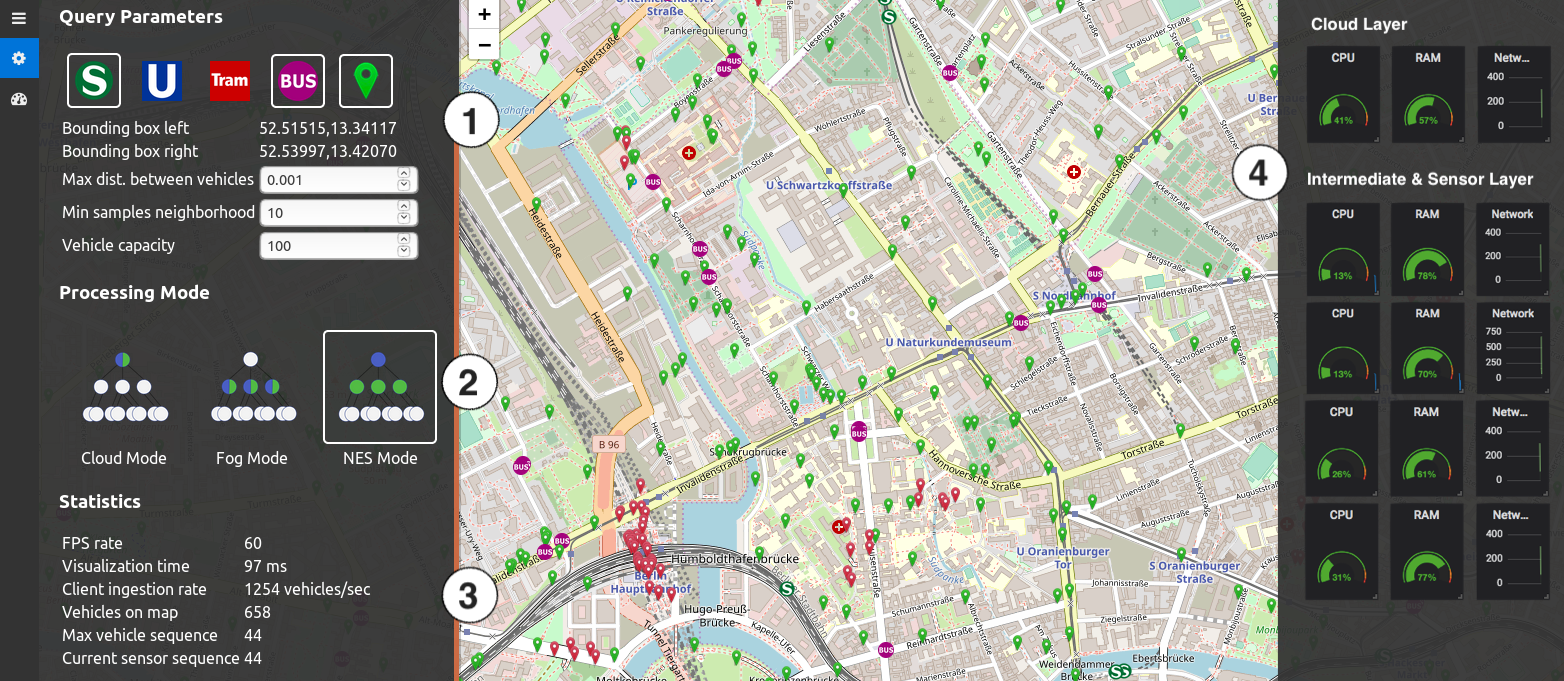
\includegraphics[width=\textwidth]{figs/MapWithClusters_Metrics.png}
  \caption{Demo GUI with potential passengers, buses, and trains. The application clusters potential passengers (green) by area density, and marks clusters red for insufficiently covered areas. The visitor may configure the query parameters (1), the processing modes (2), and observe query information (3) and runtime statistics about resource utilization (4).}
  \label{fig:screenshot}
\end{figure*}


%with the help of DBSCAN \cite{Ester:1996:DAD:3001460.3001507}. DBSCAN clusters the input data based on their closeness. It also provides two parameters to change how DBSCAN defines which objects are close to one another. The first parameter represents the maximal possible distance between two samples, while the second accounts for the minimum number of samples in the neighborhood of a core point. A visitor may change both to explore various cluster scenarios. \\ 

\subsection{Demo Setup}
\label{subsec:setup}

In the following, we describe the setup of our demonstration.

\textbf{Hardware:} For our demonstration scenario, we assume a topology where each public transport vehicle carries a sensor, which transmits its geolocation to a base station, at regular time intervals. Potential passengers also send their geolocation to the base stations, e.g., with a mobile application that uses the sensor attached to a mobile phone. 
For demonstration purposes, we use Raspberry Pis as base stations (fog nodes), and a Laptop as a cloud node. The nodes are interconnected through a router.

\textbf{Software:} Our application consists of a user frontend, and a webserver which uses NES as its execution engine for data processing. The webserver acts as an intermediator between multiple user frontends, and NES. It coordinates query transmission to NES, and forwards query results to our frontends.
Our application backend is written in Python, and uses the Flask microframework. The frontend is implemented in Javascript, and utilizes websockets to communicate with the webserver. We employ the Leaflet framework to implement our interactive map.

\textbf{Dataset:} We simulated two sensor types to compose the dataset for our demonstration.
First, we simulate vehicle sensor data directly at the base stations using real-world \textit{General Transit Feed Specification} datasets~\cite{gtfs}.
Second, we simulate potential passengers using the \textit{Simulation of Urban Mobility} (SUMO) generator~\cite{sumo}. 
We partition both datasets by geolocation, to resemble geographically distributed base stations.
The sensor records contain the measured time, and information about each measurement, such as sensor geolocation, and vehicle type. \textcolor{red}{Laura: Each measurement passt hier irgendwie nicht so gut. Vielleicht lieber: ... and additional information, such as sensor geolocation ...}

\subsection{Application}
\label{section:application}
In our demonstration, we highlight two aspects of a data management system for the IoT.
First, we showcase the deployment process that takes submitted ad-hoc queries from a user interface as input, and deploys operators on the processing nodes to answer this query.
Secondly, we demonstrate the query execution process in NES, by deploying different execution plans, and revealing their implications on resource utilization.
% We use the remainder of this section to further describe those aspects.

\subsubsection{Query Deployment}
%The use case of this application is to detect underserved areas based on crowdedness. 
%We show NES's potential as we deploy the visitor's inputs from the application's interface to NES queries by reducing data as early as possible in the IoT Network. Especially in visualization scenarios reducing data is key for performance issues as well as responsiveness. To fulfill this purpose, NES provides the possibility to filter data needed for visualization purposes as early as in the Fog Layer. Therefore, it not only reduces the data send to the visualization application but the overall network traffic.
%Once a user interacts with the GUI, NES receives a query including parameters for the following three operations:
% 
The main goal of our application is to detect underserved areas based on crowdedness. 
In this application, NES allows us to reduce data as early as possible in the IoT infrastructure. 
Especially in visualization scenarios, data reduction is a key performance factor, and naturally occurs because users are seldomly interested in the entire data set.
To this end, NES provides the option to filter data needed for visualization purposes already in the intermediate (fog) layer. 
The resulting data reduction is two-fold. 
First, NES uses on-demand data acquisition techniques to only gather sensor data that is currently required to answer the query.
Seconds, NES uses intermediate nodes to evict unnecessary data close to the sensors.
Both data reductions minimize the overall network traffic inside the IoT infrastructure, as well as data that has to be sent to applications, in our case the web server.

In our demonstration, the application sends a new query to NES, every time a visitor interacts with the map and its options. A visitor interaction on the map creates a new query that consists of the following parametrized operations:
\begin{itemize}
  \item \textbf{Map Bounding Box:} This parameter filters \textcolor{red}{Laura: These parameters filter ... (es sind ja mehrere Parameter)} the vehicles, and potential passengers located within a bounding box. The bounding box depends on the map area currently viewed by the visitor.
  \item \textbf{Vehicles and Passengers:} This parameter \textcolor{red}{Laura: Same as above} filters passengers, and selected vehicle types, e.g., bus, train, or subway.
  \item \textbf{Clustering:} This parameter adjusts \textcolor{red}{Laura: Same as above} the specifications for our clustering algorithm (DBSCAN~\cite{dbscan}), such as object distance. The algorithm clusters the previously filtered sensor records, and yields the underserved areas. 
\end{itemize}

%Therefore, NES retrieves information to reduce the data load from the interface through queries. 
%Every time a visitor interacts with the map and its options, the application sends a new query to NES. Those queries include parameters to define the currently selected map part, and visitor's selection of vehicle types. 
%In each case, NES limits the processed and send data load to adhere to the requested parameters. 
% We implement our crowdedness algorithm and filtering operations on NES, which reduces the data amounts transferred to the user interface.
% The application itself includes a webserver, that is accessible by multiple clients, i.e. web browsers.
% Mapping the user interface with queries
%NES takes this query and applies it onto the given topology.
% NES takes care of data management operations, while in the application we focus only on implementing the business logic.%, in our case filtering vehicles and highlighting crowded clusters.
%In our application, we use NES as a data management backend, and forward only necessary data to our application.
% 
\subsubsection{Query Execution}
% 
In \Cref{nes}, we introduced the NES Optimizer, which produces, and evaluates potential execution plans.
Each execution plan contains a mapping of NES operators to nodes in the IoT infrastructure.
The optimizer would come up with three execution plans that resemble cloud-based, fog-based, and unified approaches, which we refer to as processing modes.
Note that in our demonstration, we use NES to reproduce all processing modes.
% 
In ~\Cref{fig:screenshot}~\circled{2}, we present these modes, marking filter operations with green color, and clustering operations with blue color.
In our demonstration, visitors can choose between the following three processing modes:
%\nointent 
% \begin{figure*}[t!]
%   \centering
%    \begin{subfigure}[t]{0.339\textwidth}
%         \centering
%         \includegraphics[width=\textwidth]{figs/Cloud_mode_ut.png}
%         \caption{Cloud Mode.}
%     \end{subfigure}%
%     ~ 
%     \begin{subfigure}[t]{0.28\textwidth}
%         \centering
%         \includegraphics[width=\textwidth]{figs/Fog_mode_ut.png}
%         \caption{Fog Mode.}
%     \end{subfigure}%
%     ~ 
%     \begin{subfigure}[t]{0.277\textwidth}
%         \centering
%         \includegraphics[width=\textwidth]{figs/NES_mode.png}
%         \caption{NES Mode.}
%     \end{subfigure}%
%   \caption{Processing modes supported by NES. Green nodes process the filter operation. Blue nodes process the clustering operation. Red nodes represent high CPU and RAM utilization. Red connections mark high incoming network traffic.}
%   \label{fig:execution-plans}
% \end{figure*}

\begin{itemize}
  \item \textbf{Cloud Mode:} The cloud mode represents the processing of current cloud-based SPEs. NES places all operators on the cloud nodes. Performance metrics will reveal that the main workload gathers in the cloud layer while the processing resources of the intermediate fog nodes remain unused.
  \item \textbf{Fog Mode:} NES places all operators on the intermediate layer. The visitor will observe that filtering on the fog reduces network traffic. However, CPU, and RAM usage on the fog nodes increases significantly.
  \item \textbf{NES Mode:} NES places the filter operators on the fog nodes, and the clustering operator on the cloud nodes. The visitor will observe that network traffic, CPU, and RAM utilization remain at a moderate level due to evenly distributed workloads alongside the early filters.
\end{itemize}

In sum, in this demonstration, we highlight the shortcomings of state-of-the-art systems for IoT applications, and the benefits of using NES as a data management platform for IoT scenarios. \textcolor{red}{Laura: Der Satz passt meines Erachtens nach eher in die Conclusion als hier hin, da wir in dieser Sektion nicht auf die shortcomings bzw. benefits von NES eingehen.}
%\textbf{IoT Monitoring.}
%A visitor can monitor the incoming network traffic, RAM and CPU utilization per node on the right in Figure~\ref{fig:screenshot}. %Incoming tuples, 
%The visitor can see: 
% - RAM utilization
% - CPU utilization
% - Tuples incoming
% - Data Ingestion
% of the intermediate layer and the cloud layer.

%\nointent 
%\textbf{Logical Plan}
%- Multiple users/queries are supported.
%- Filtering by Window size. 
%- Filtering by Trasport type.
%- Clustering

%\noindent \textbf{Interactions.} The application can be configured to operate in different modi, in order to allow the visitor to observe performance metrics of various deployment strategies, e.g. saved network traffic during filter push-down. Furthermore, everytime the map is moved, we deploy a new query with the new bounding box parameters, and the new stream is seamlessly ingested by our application.
